%\documentclass[10pt, twocolumn]{article}
%\documentclass[11pt]{article}
%\documentclass[twocolumn,showpacs,preprintnumbers,amsmath,amssymb,prl, superscriptaddress]{revtex4}
%\documentclass[twocolumn, preprintnumbers,amsmath,amssymb,prd, superscriptaddress]{revtex4}
\documentclass[preprintnumbers,amsmath,amssymb,prd,superscriptaddress]{revtex4}
%\documentclass[10pt, preprint,showpacs,preprintnumbers,amsmath,amssymb, superscriptaddress]{revtex4}
%\documentclass[11pt, prd,preprintnumbers,amsmath,amssymb, superscriptaddress]{revtex4}
%\documentclass[11pt, prd,preprintnumbers, amsmath,amssymb, superscriptaddress, nofootinbib, hyperref]{revtex4}

\usepackage{latexsym}
\usepackage{amssymb}
\usepackage{epsfig,amsmath,graphics}
\usepackage{epstopdf}
\usepackage{verbatim}
\usepackage{wasysym}
\usepackage{hyperref}
\usepackage{feynmp-auto} % feynman diagrams
%\usepackage{subfig}
\usepackage[utf8]{inputenc}
\usepackage{xpatch}
\usepackage{xcolor}
\usepackage{mathtools}
\hypersetup{
    colorlinks,
    linkcolor={red!80!black},
    citecolor={green!60!black},
    urlcolor={blue!60!black}
}
\usepackage{appendix}

\newcommand{\Ez}{\mathcal{E}_0}
\newcommand{\Eboom}{\mathcal{E}_\text{boom}}
\newcommand{\OO}{\mathcal{O}}
\newcommand{\LL}{\mathcal{L}}
\newcommand{\HH}{\mathcal{H}}
\newcommand{\TeV}{\text{TeV}}
\newcommand{\GeV}{\text{GeV}}
\newcommand{\MeV}{\text{MeV}}
\newcommand{\keV}{\text{keV}}
\newcommand{\rad}{\text{rad}}
\newcommand{\cm}{\text{cm}}
\newcommand{\angstrom}{\buildrel _{\circ} \over {\mathrm{A}}}
\newcommand{\pslash}{p\hspace{-0.070in}/\,}
\newcommand{\Mpl}{M_{\text{pl}}}
\newcommand{\ket}[1]{\ensuremath{\left|#1\right>}}
\newcommand{\bra}[1]{\ensuremath{\left<#1\right|}}
\newcommand{\braket}[2]{\ensuremath{\left<#1|#2\right>}}
%Large Parentheses
\def\r{\right)}
\def\l{\left(}

\begin{document}

%\preprint{APS/123-QED}

\subsection{Transits}

\paragraph{Boom Condition.}
The energy deposited during a continuous heating event such as a DM transit is best described in terms of a linear energy transfer $(dE/dx)_\text{LET}$, the kinetic energy of SM particles produced per distance traveled by the DM.
If these products have a heating length $L_0$ then the relevant energy deposit must at minimum be taken as the energy transferred over the transit distance $L_0$.
Of course, we can always choose to consider energy deposits over a longer segment of the DM trajectory.
Importantly, as per the general condition \eqref{eq:energy_boom_condition} such a deposition is \emph{less} explosive unless $L_0$ is smaller than the trigger size $\lambda_T$.
Thus, we consider the energy deposited in a transit over the larger of these two length scales.
Assuming the energy of the DM is roughly constant over this heating event, the boom condition for transit heating is:
\begin{align}
\label{eq:transitexplosion}
  \left( \frac{d E}{d x} \right)_\text{LET} \gtrsim
  \frac{\Eboom}{\lambda_T} \cdot \text{Max}
  \left\{\frac{L_0}{\lambda_T}, 1 \right\}^2.
\end{align}

The above argument sums the individual energy deposits along the DM trajectory as though they are all deposited simultaneously.
This is possible if the DM moves sufficiently quickly so that this energy does not diffuse out of the region of interest before the DM has traversed the region.
We therefore require that the diffusion time $\tau_\text{diff} \approx 10^{-12} ~\text{s}$ across a heated region at temperature $T_f$ be larger than the DM crossing-time:
\begin{align}
  \tau_\text{diff} \sim \frac{L^2}{\alpha(T_f)} \gg
  \frac{L}{v_\text{esc}},
\label{eq:SlowDiffusion}
\end{align}
where $\alpha(T)$ is the temperature-dependent diffusivity, and the DM transits at the stellar escape velocity $v_\text{esc} \approx 10^{-2}$.
This condition is more stringent for smaller regions, so we focus on the smallest region of interest, $L = \lambda_T$.
\eqref{eq:SlowDiffusion} is then equivalent to demanding that the escape speed is greater than the conductive speed of the fusion wave front, $v_\text{cond} \sim \alpha(T_f) / \lambda_T$.
Numerical calculations of $v_\text{cond}$ are tabulated in \cite{Woosley}, and indeed condition \eqref{eq:SlowDiffusion} is satisfied for all WD densities.

\paragraph{Event Rate: Wind Scenario.}
The rate of transit events is given by the flux of DM passing through a WD
\begin{align}
  \Gamma_\text{transit} \sim
  \frac{\rho_{\chi}}{m_\chi} R_\text{WD}^2
  \l\frac{v_\text{esc}}{v_\text{halo}}\r^2 v_\text{halo},
\label{eq:TransitFluxCondition}
\end{align}
where $m_\chi$ is the DM mass, $\rho_\chi$ is the local DM density near the WD, and $R_\text{WD} \approx 4000 ~\text{km}$ is the WD radius.
Here $v_\text{halo} \sim 10^{-3}$ is galactic virial velocity, and the transit rate contains an $\OO(100)$ enhancement due to gravitational focusing.

\paragraph{WD Shielding.}
Runaway fusion only occurs in the degenerate WD interior where thermal expansion is suppressed as a cooling mechanism.
The outer layers of the WD, however, are composed of a non-degenerate gas and it is therefore essential that a DM candidate penetrate this layer in order to ignite a SN.
We parameterize this by a DM stopping power $(dE/dx)_\text{SP}$, the kinetic energy lost by the DM per distance traveled in the non-degenerate layer, and demand that
\begin{align}
\label{eq:CrustCondition}
  \left( \frac{d E}{d x} \right)_\text{SP} \ll
  \frac{m_\chi v^2_\text{esc}}{R_\text{envelope}},
\end{align}
where $R_\text{envelope} \approx 50 ~\text{km}$ is the width of a WD envelope \cite{KippenhahnWeigert}.
Note that the DM stopping power in the non-degenerate layer $(dE/dx)_\text{SP}$ and the linear energy transfer in the degenerate interior $(dE/dx)_\text{LET}$ are possibly controlled by different physics and may have very different numerical values.
In addition, a transit heating event satisfying condition \eqref{eq:CrustCondition} will have negligible energy loss over the parametrically smaller trigger size or heating length $L_0$, validating the boom condition \eqref{eq:transitexplosion}.

\subsection{Collisions and Decays}

\paragraph{Boom Condition.}
For a point-like DM-DM collision or DM decay event releasing particles of heating length $L_0$, ignition will occur if the total energy in SM products satisfies condition~\eqref{eq:energy_boom_condition}.
Such an event will likely result in both SM and dark sector products, so we parameterize the resulting energy in SM particles as a fraction $f_\text{SM}$ of the DM mass.
For non-relativistic DM, the DM mass is the dominant source of energy and therefore $f_\text{SM} \lesssim 1$ regardless of the interaction details, although we may well suspect that $f_\text{SM} \ll 1$ for realistic models.
With this parameterization, a single DM-DM collision or DM decay has a boom condition:
\begin{equation}
\label{eq:coldecay}
  m_\chi f_\text{SM}  \gtrsim \Eboom \cdot \text{max} \left \{\frac{L_0}{\lambda_T}, 1 \right \}^3.
\end{equation}
We are thus sensitive to DM masses $m_\chi \gtrsim 10^{16} ~\GeV$.

However, there is an interesting possibility if DM is captured in the WD that allows collisions of lower mass DM to ignite the star. 
Multiple DM-DM collisions in a sufficiently small region can occur rapidly enough to be counted as a single heating event.
This is similar in nature to a transit heating event, where multiple scatters across a transit length $\lambda_T$ can release an energy $\Eboom$ and satisfy \eqref{eq:transitexplosion} even if any individual scatter is not explosive by itself.   
If a single DM-DM collision is unable to ignite the star, the sum total of the energy released in many collisions can still result in a SN if the following boom condition is satisfied:
\begin{equation}
\label{eq:multcolboom}
 m_\chi f_\text{SM}  \gtrsim \frac{\Eboom}{N_\text{mult}} \cdot \text{max} \left \{\frac{L_0}{\lambda_T}, 1 \right \}^3, ~~~~ N_\text{mult} \gtrsim 1. 
\end{equation}
We define $N_\text{mult}$ as the number of collisions happening within a region of size $\text{max}\{\lambda_T,L_0\}^3$ (or smaller) during a diffusion time $\tau_\text{diff}$.
This necessarily depends on the DM-DM collision cross section, the DM-SM scattering cross section, and the evolution of the captured DM in the star. 
As we will see, the condition for multiple collisions to be explosive \eqref{eq:multcolboom} contains a number of additional assumptions about the DM and its interactions that are not present for a single, explosive collision. 
These are discussed in detail below. 

\paragraph{Event Rate: DM Wind.}
DM with negligible energy loss in the WD medium will traverse the star in $\sim R_\text{WD}/v_\text{esc} \approx 0.1 ~\text{s}$ and have a number density within the WD enhanced relative to the average galactic density by a factor $(v_\text{esc}/v_\text{halo}) \sim 10$.
In the wind scenario, the DM-DM collision rate inside the WD parameterized by a cross-section $\sigma_{\chi \chi}$ is:
\begin{align}
  \Gamma_\text{collision}
  \sim \l \frac{\rho_\chi}{m_\chi} \r^2 \sigma_{\chi \chi} \l \frac{v_\text{esc}}{v_\text{halo}}\r^3 v_\text{halo} R_\text{WD}^3.
  \label{eq:collisionDM}
\end{align}
Similarly the net DM decay rate inside the WD parameterized by a lifetime $\tau_\chi$ is:
\begin{align}
 \Gamma_\text{decay}
   \sim \frac{1}{\tau_\chi} \frac{\rho_{\chi}}{m_\chi} \l \frac{v_\text{esc}}{v_\text{halo}}\r R_\text{WD}^3.
  \label{eq:decayDM}
\end{align}

\paragraph{Event Rate: DM Capture.}
For the DM to be captured in a WD, it must have sufficiently strong interactions with stellar constituents:
\begin{equation}
\label{eq:capture}
\left( \frac{d E}{d x} \right)_\text{SP} \gtrsim \frac{m_\chi v^2}{R_\text{WD}},
\end{equation}
where $v \in [0, 2 v_\text{halo}]$ is the DM galactic virial velocity relative to the WD.  
For $v \ll v_\text{esc}$, we demand that the DM lose a fraction $(v/v_\text{esc})^2$ of its energy to eventually become stopped in the star. 
Of course, the most probable relative velocity is of order $v_\text{halo} \sim 10^{-3}$.
The distribution of DM particles at relative velocity $v$ is given by:
\begin{equation}
\frac{dn}{dv} \sim \frac{\rho_\chi}{m_\chi} \frac{v}{v_\text{halo}^2},
\end{equation}
appropriately normalized. 
If every DM that passes through the WD is captured, then the capture rate $\Gamma_\text{cap}$ is simply \eqref{eq:TransitFluxCondition}. 
However even if the interaction is unable to capture DM at a velocity $v_\text{halo}$, it may still capture those DM with a lower relative velocity.
The capture rate is roughly
\begin{equation}
\Gamma_\text{cap} \sim \Gamma_\text{transit} \cdot \text{min} \left \{ \frac{v_\text{cap}}{v_\text{halo}}, 1\right \}. 
\end{equation}
where $v_\text{cap}$ is the velocity below which the DM-SM interaction is capable of capturing the DM. 

For the remainder of this section, all numerical quantities are evaluated assuming a WD lifetime $\tau_\text{WD} \sim 5 ~\text{Gyr}$ and central WD density $n_\text{ion} \sim 10^{31} ~\cm^{-3}$. 
At this density, the relevant WD parameters are approximately: 
\begin{equation}
v_\text{esc} \approx 3 \times 10^{-2}, ~~~~ R_\text{WD} \approx 4000 ~\text{km}, ~~~~ M_\text{WD} \approx 1.25 ~M_{\astrosun}. 
\end{equation}

The physics of DM capture can be made more precise for a specific interaction.
The simplest scenario is a spin-independent, elastic scattering off ions characterized by cross section $\sigma_{\chi A}$. 
For $m_\chi \gg m_\text{ion}$, the typical momentum transfer in an elastic scatter is $q \sim \mu_{A} v_\text{esc} \approx 300 ~\MeV$, where $\mu_{A}$ is the reduced mass of the DM-ion system. 
The typical energy transfer in a nuclear elastic scatter is simply $q^2/m_\text{ion} \sim m_\text{ion} v_\text{esc}^2 \approx 10 ~\MeV$. 
Evidently, the DM is capable of losing the necessary fraction of its energy for capture after a single elastic scatter if
\begin{equation}
m_\chi \lesssim m_\text{ion} \l \frac{v_\text{esc}}{v} \r^2 \approx 10^4 ~\GeV \l \frac{10^{-3}}{v} \r^2
\end{equation}
In the case of multiple scatters, the stopping power of the DM is
\begin{equation}
\left( \frac{d E}{d x} \right)_\text{SP} \sim n_\text{ion} \sigma_{\chi A} m_\text{ion} v^2.
\end{equation}
Demanding \eqref{eq:capture} yields a condition on the DM elastic nuclear cross section sufficient for capture:
\begin{equation}
\label{eq:capturecross}
\sigma_{\chi A} \gtrsim  \l \frac{m_\chi}{m_\text{ion}} \r \l \frac{v}{v_\text{esc}} \r^2 \frac{1}{n_\text{ion}} \frac{1}{R_\text{WD}} \approx 10^{-38} ~\cm^2 \l \frac{m_\chi}{10^{6} ~\GeV} \r \l \frac{v}{10^{-3}} \r^2,
\end{equation}
Thus, DM with velocities less than
\begin{equation}
v_\text{cap}^2 \sim v_\text{esc}^2 \sigma_{\chi A} \l \frac{m_\text{ion}}{m_\chi} \r n_\text{ion} R_\text{WD} 
\end{equation}
are sufficiently captured by the WD. 
Evidently, the assumption that the scatters responsible for slowing the DM are not sufficient to blow up the WD \eqref{eq:transitexplosion} is a valid one if the cross section satisfies
\begin{equation}
\sigma_{\chi A} < \l \frac{\Eboom}{\lambda_T} \r \l \frac{1}{m_\text{ion} v_\text{esc}^2} \r \l \frac{1}{n_\text{ion}} \r \approx 10^{-8} ~\cm^2,
\end{equation}
Since the momentum transfer $q$ is roughly of order the inverse nuclear size, it is reasonable to expect the DM coherently scatters off all nucleons in the nucleus. 
The average per-nucleon cross section (spin-independent) is
\begin{equation}
\sigma_{\chi A} = A^2 \l \frac{\mu_{A}}{\mu_{n}}\r^2 F^2(q) \sigma_{\chi n} \sim A^4 F^2(q) \sigma_{\chi n},
\end{equation}
where $F^2(q) \sim 10^{-2}-10^{-1}$ is the Helm form factor, calculated based on the analytic expression in \cite{LUX thesis}. 
Thus, the cross section sufficient for capture
\begin{equation}
\sigma_{\chi n} \gtrsim 10^{-41} ~\cm^2 \l \frac{m_\chi}{10^{6} ~\GeV} \r \l \frac{v}{10^{-3}} \r^2
\end{equation}
can be compared to limits from direct detection experiments. 
Currently, the most stringent bound on DM nuclear elastic scatters comes from XENON 1T:
\begin{equation}
\label{eq:xenon}
\sigma^\text{XENON}_{\chi n} < 10^{-42} ~\text{cm}^2 \l \frac{m_\chi}{10^6 ~\GeV} \r.
\end{equation}
Evidently, direct detection bounds constrain the capture of DM in WDs via elastic scatters.

We now review the evolution of DM within the star once it has been captured. 
The DM eventually thermalizes at a velocity
\begin{equation}
v_\text{th} \sim \sqrt{\frac{T}{m_\chi}} \approx 10^{-12} \l \frac{10^{16} ~\GeV}{m_\chi}\r^{1/2},
\end{equation}
where $T \sim \keV$ is the WD temperature.
At this point, the DM accumulates at the radius where its kinetic energy balances against the gravitational potential energy of the enclosed WD mass:
\begin{align}
  R_\text{th} \sim \l \frac{T}{G m_\chi \rho_\text{WD}}\r^{1/2} \approx 0.1 ~\cm \l \frac{10^{16} ~\GeV}{m_\chi}\r^{1/2}
\end{align}
where we have assumed a constant WD density $\rho_\text{WD} \sim n_\text{ion} m_\text{ion}$ within $R_\text{th}$.
Of course, the timescale for captured DM to thermalize and settle at $R_\text{th}$ depends on the nature of the DM-SM interaction.
If the DM is capable of losing energy rapidly in the star, we expect this time to be of order
\begin{align}
\label{eq:tdrift}
  t_\text{settle} \sim \frac{R_\text{WD}}{v_\text{th}}
  \approx 50 ~\text{yr} \l \frac{m_\chi}{10^{16} ~\GeV} \r^{1/2}. 
\end{align}
The settle time can be explicitly calculated in the case that the DM is captured via elastic nuclear scatters. 
We simply demand that the settle time is shorter than the age of the WD:
\begin{equation}
t_\text{settle} < \tau_\text{WD}.
\end{equation}
Note that the in-falling DM constitutes a number density of DM throughout the WD volume.
%\begin{equation}
%n(r) \sim \frac{\Gamma_\text{cap}}{r^2 v(r)}.
%\end{equation}
Integrating over the WD, the total annihilation rate for the in-falling DM is of order
\begin{equation}
\label{eq:infallrate}
\Gamma_\text{infall} \sim \frac{\Gamma_\text{cap}^2 \sigma_{\chi \chi}}{R_\text{th} v_\text{th}}.
\end{equation}
We can ignore the depletion of in-falling DM as long as \eqref{eq:infallrate} is less than the capture rate:
\begin{equation}
\label{eq:steadycollect}
\Gamma_\text{infall} < \Gamma_\text{cap}.
\end{equation}
In the case of efficient capture $\Gamma_\text{cap} \sim \Gamma_\text{trans}$, condition \eqref{eq:steadycollect} is independent of $m_\chi$ and translates to an upper bound on the cross section $\sigma_{\chi \chi} < 10^{-13} ~\text{cm}^2$. 

After the initial off-set time $t_\text{settle}$, DM will begin steadily collecting at the thermal radius.
Assuming \eqref{eq:steadycollect} is satisfied, the collection rate is roughly the same as the capture rate $\Gamma_\text{cap}$. 
However, the DM is also annihilating with itself.
Eventually, the collection and annihilation rates become comparable and there is an equilibrium number of DM particles accumulated at the thermal radius:
\begin{align}
N_\text{eq} \sim \l \frac{\Gamma_\text{cap} R_\text{th}^3}{\sigma_{\chi \chi} v_\text{th}} \r^{1/2} \approx 10^{19} \l \frac{10^{16} ~\GeV}{m_\chi} \r \l \frac{10^{-30} ~\cm^2}{\sigma_{\chi \chi}} \r^{1/2} \l \frac{\rho_\chi}{0.4 ~\GeV/\cm^3} \r^{1/2}.
\end{align}
Of course, there is no guarantee that this equilibrium state is achieved within the age of the WD. 
In that case, we can ignore annihilations and the total number of DM particles accumulated is simply
\begin{align}
N_\text{life} &\sim \Gamma_\text{cap} \tau_\text{WD} \approx 10^{29}  \l \frac{10^{16} ~\GeV}{m_\chi} \r \l \frac{\rho_\chi}{0.4 ~\GeV/\cm^3} \r
\end{align}
As expected, the total \emph{mass} of DM that the WD can possibly accumulate is independent of DM mass $M_\text{life} \sim 10^{45} ~\GeV \ll M_\text{WD}$. 
However, if the collected mass of DM at the thermal radius ever exceeds the WD mass within this volume, then there is the possibility of self-gravitational collapse of the DM.
The critical number of DM particles needed for collapse is given by
\begin{align}
\label{eq:Ncore}
    N_\text{crit} \sim \frac{\rho_\text{WD} R^3_\text{th}}{m_\chi} \approx 10^{12} \l \frac{10^{16} ~\GeV}{m_\chi} \r^{5/2}. \nonumber
\end{align}
This can only be achieved if the time to collect a critical mass of DM is shorter than the time for annihilations to deplete this mass sufficiently \emph{and} shorter than the WD lifetime. 
In other words:
\begin{equation}
\label{eq:collapsecondition}
N_\text{crit} < N_\text{eq}, ~~~~ N_\text{crit} < N_\text{life}.
\end{equation}
Importantly, we see that DM masses less than $\sim 10^{6} ~\GeV$ do not have enough time within the age of the WD in a DM density $\rho_\chi \sim 0.4 ~\GeV/\cm^3$ to collect a number $N_\text{crit}$ and begin a collapse. 
At a given radius $r$, the time it takes for the DM to free-fall an $\OO(1)$ fraction of this distance is roughly
\begin{equation}
\label{eq:freefalltime}
t_\text{ff} \sim \frac{r}{v_\text{ff}}, ~~~~ v_\text{ff} \sim \sqrt{\frac{G N m_\chi}{r}}.
\end{equation}
Thus, the timescale for self-gravitational collapse at the thermal radius is independent of DM mass:
\begin{align}
\label{eq:collapsetime}
  t_\text{collapse} \sim \frac{R_\text{th}}{v_\text{th}} \approx 0.1 ~\text{s}.
\end{align}
Of course, it is possible that the DM initially remains thermalized while collapsing due to sufficiently strong DM-SM interactions. 
In the case of elastic nuclear scatters, the collapsing DM is instead free-falling at the thermal radius if
\begin{equation}
\sigma_{\chi n} \lesssim \frac{1}{n_\text{ion} R_\text{th}} \l \frac{m_\chi}{m_\text{ion}}\r \approx 10^{-33} ~\cm^2 \l \frac{m_\chi}{10^6 ~\GeV} \r^{3/2},
\end{equation}
which is necessarily the case for any cross sections which satisfy the XENON bound. 
Depletion of the collapsing DM mass becomes important when the timescale for collapse is of order the timescale for annihilation, which occurs at a radius
\begin{align}
R_{\chi \chi} \sim \sqrt{N_\text{crit} \sigma_{\chi \chi}} \approx 10^{-9} ~\cm  \l \frac{10^{16} ~\GeV}{m_\chi} \r^{5/4} \l \frac{\sigma_{\chi \chi}}{10^{-30} ~\cm^2} \r^{1/2}. 
\end{align}
This can be seen explicitly by solving the differential equation for the total rate of annihilations in the collapsing volume:
\begin{equation}
\label{eq:DMcollapsedeplete}
\frac{dN}{dr} \sim \frac{N^2}{r^3} \sigma_{\chi \chi} \Rightarrow N(r) \approx \frac{N_\text{crit}}{1+ R_{\chi \chi}^2 \l \frac{1}{r^2} -\frac{1}{R_\text{th}^2}\r}
\end{equation}
Thus, below $R_{\chi \chi}$ the number (and mass) of collapsing DM depletes as $N(r) \propto r^2$. 
This is only sensible if the DM collapses below the thermal radius (so we are justified calling the evolving DM density profile a ``collapse"):
\begin{align}
\label{eq:xicondition}
R_{\chi \chi} < R_\text{th}.
\end{align}
%It turns out condition \eqref{eq:xicondition} is always true if both \eqref{eq:collapsecondition} and the associated boom condition \eqref{eq:multcolboom}, described in detail below, are satisfied. 

There are two potential evolutions of the captured DM: either the DM collapses or it does not. 
For the later, it must be that the DM has reached its equilibrated number at the thermal radius or is still continuing to accumulate, not yet having the critical mass necessary for collapse within its lifetime:
\begin{equation}
\label{eq:nocollapseann}
\text{min}\{N_\text{eq}, N_\text{life}\} < N_\text{crit}.
\end{equation}
Turning towards the boom condition for multiple collisions \eqref{eq:multcolboom}, the number of collisions taking place in a trigger-sized subregion of $R_\text{th}$ within a time $\tau_\text{diff}$ is roughly:
\begin{equation}
\label{eq:nocollapse}
N_\text{multi} \sim \l \frac{\text{min}\{N_\text{eq}, N_\text{life}\}}{R_\text{th}^3} \r^2 \sigma_{\chi \chi} v_\text{th} \text{max}\{\lambda_T,L_0\}^3 \tau_\text{diff}. 
\end{equation}
As an example, consider the case in which the DM is efficiently captured by the WD $v_\text{cap} \sim v_\text{halo}$. 
Even in this ``best-case" scenario, we find that there is no available parameter space $\{m_\chi, \sigma_{\chi \chi}\}$ where both \eqref{eq:nocollapseann} and \eqref{eq:multcolboom}---with $N_\text{multi}$ given by \eqref{eq:nocollapse}---are simultaneously satisfied. 

Therefore, we instead turn our attention to collapsing DM, characterized by \eqref{eq:collapsecondition}. 
Of course, the number of DM-DM collisions $N_\text{multi}$ that can be counted as a single heating event depends on the where we examine the collapse. 
In general, this is given as an integral of the annihilation rate
\begin{equation}
\label{eq:capintegral}
N_\text{multi} \sim \int \l \frac{N}{r^3}\r^2 \sigma_{\chi \chi} \text{min}\{L_\text{heat}, r\}^3 dr, ~~~~ L_\text{heat} \equiv \text{max}\{\lambda_T, L_0\}
\end{equation}
integrating over the distance fell within a fixed time interval $\tau_\text{diff}$. 
The expectation is that there exists an optimal value of the lower radius at which $N_\text{multi}$ is maximized.
We denote this as $R_*$. 
However, even without knowing the details of this optimum choice, we can calculate \eqref{eq:capintegral} by considering the following limits. 
If the free-fall time \eqref{eq:freefalltime} at a distance of order $R_*$ is much larger than the diffusion time, the annihilation rate can be approximated as constant over a time $\tau_\text{diff}$.
If this free-fall time is instead much smaller than the diffusion time, the annihilation rate is a rapidly increasing function over the interval $\tau_\text{diff}$.
Therefore, \eqref{eq:capintegral} is approximated by the peak value of the annihilation rate (which is maximized at $R_*$) multiplied by the time spent at this peak (which is the time to free-fall $\sim R_*$).
Considering both these possibilities, the maximum value of \eqref{eq:capintegral} is of the form: 
\begin{equation}
\label{eq:nmulti}
N_\text{multi} \sim \l \frac{N}{R_*^3}\r^2  \sigma_{\chi \chi} v_\text{ff} ~\text{min}\{L_\text{heat}, R_*\}^3 ~\text{min}\{\tau_\text{diff}, R_*/v_\text{ff}\},
\end{equation}
The questions is: what is $R_*$?
Ultimately, the answer depends on the parameters $m_\chi$ and $\sigma_{\chi \chi}$. 
If $R_{\chi \chi} > L_\text{heat}$, then clearly $N_\text{multi}$ is maximized at $R_* \sim L_\text{heat}$.
On the other hand, if $R_{\chi \chi} < L_\text{heat}$ then $N_\text{multi}$ is maximized at $R_* \sim R_{\chi \chi}$.
However, there may be some stabilizing pressure which prevents the DM from collapsing below a radius $R_\text{sta}$.
This is reasonable to expect in the case of composite DM, although such a stable radius necessarily depends on unknown physics. 
In any case, the optimum radius is determined as follows:
\begin{equation}
R_* = \text{max}\{\text{min}\left \{L_\text{heat}, R_{\chi \chi}\}, R_\text{sta}\right\}.
\end{equation}

Famously, gravity itself provides such a ``pressure", arresting collapses below the Schwarzschild radius by the formation of a black hole (BH):
\begin{equation}
R_\text{BH} \sim G m_\chi N_\text{crit} \approx 5 \times 10^{-24} ~\cm \l \frac{10^{16} ~\GeV}{m_\chi} \r^{3/2}.
\end{equation}
Note that if the DM number is substantially depleting according to \eqref{eq:DMcollapsedeplete} in the case that $R_\text{BH} < R_{\chi \chi}$, then a BH never forms and the optimal radius is simply $R_* \sim L_\text{heat}$. 

\subsection{Constraints}

We now turn towards constraints on DM interactions in the capture scenario. 
In Figure \ref{fig:multicapture}, we show the constraints on DM-DM annihilation cross section $\sigma_{\chi \chi}$ into SM particles during self-gravitational collapse in a WD, i.e. multiple collisions.
We have assumed that the DM is efficiently captured, i.e. $\Gamma_\text{transit} \sim \Gamma_\text{capture}$. 
\begin{figure}
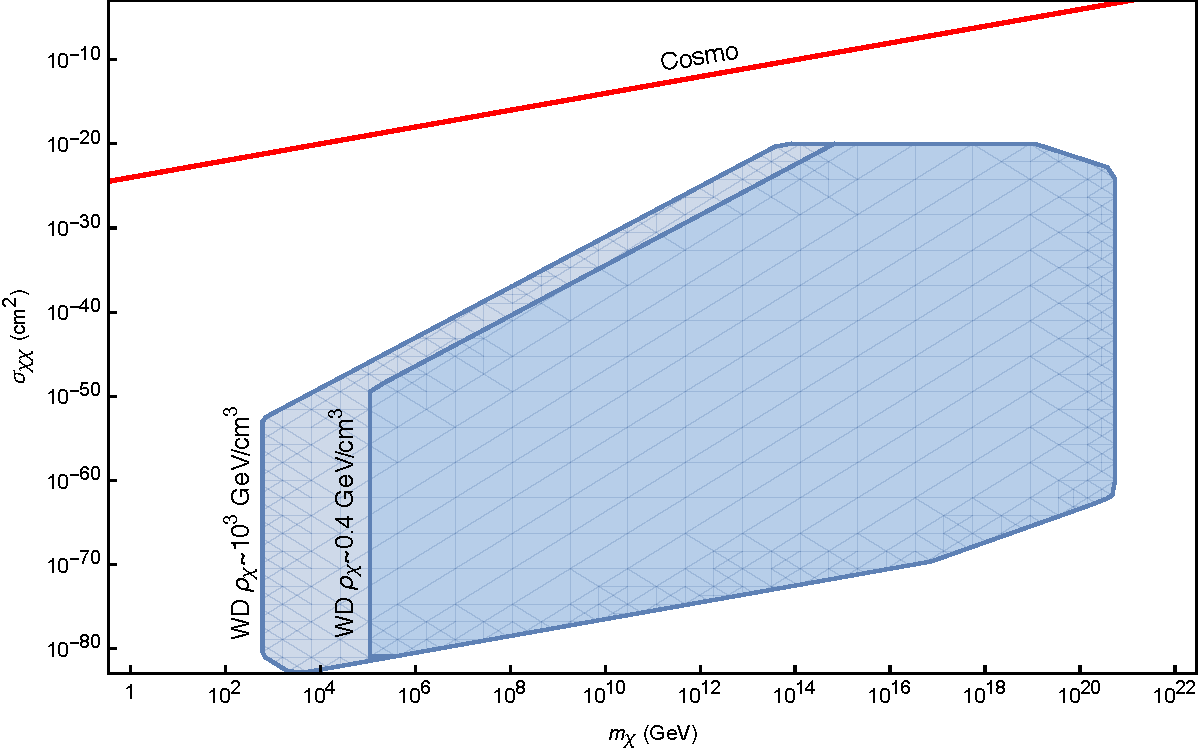
\includegraphics[scale=.35]{multicapture.pdf}
\caption{Constraints on DM-DM annihilation cross-section into SM particles which deposit their energy compactly within a trigger size $\lambda_T$ during self-gravitational collapse in a WD. Bounds come from observation of a single $1.25~M_{\astrosun}$ WD assuming efficient capture of the DM ($\Gamma_\text{cap} \sim \Gamma_\text{trans}$). We also assume the DM collapse is stabilized by formation of a BH.}
\label{fig:multicapture}
\end{figure}
The bounds in Figure \ref{fig:multicapture} are valid for any SM annihilation products which deposit their energy compactly upon release within a trigger size $\lambda_T$.
We can understand the shape of this excluded region as follows.
If the DM mass is too low, then there is not enough time within the age of the WD to collect the critical mass needed for initiating collapse.
Similarly if the cross section for annihilation is too large, then the DM will effectively deplete before reaching this critical mass. 
However, $m_\chi$ cannot be arbitrarily large or $\sigma_{\chi \chi}$ arbitrarily small---these limits are determined in a non-trivial way by the boom condition for multiple collisions \eqref{eq:multcolboom}. 
The region in Figure \ref{fig:multicapture} are the set of all points which satisfy \eqref{eq:collapsecondition} and \eqref{eq:eq:multcolboom}, with $N_\text{multi}$ given by \eqref{eq:nmulti} assuming that the DM collapse is stabilized by formation of a BH. 
Additionally, one can check that the conditions \eqref{eq:steadycollect} and \eqref{eq:xicondition} are automatically satisfied if \eqref{eq:collapsecondition} and \eqref{eq:multcolboom} are satisfied. 

Of course, the constraints on multiple DM collisions in a collapse can be made concrete for a specified DM interaction. 
As in Section \ref{sec:previous}, we consider the case where the DM is captured in a WD via elastic scatters. 
Suppose the DM scatters off nuclear targets through Z boson exchange, with a per-nucleon cross section
\begin{equation}
\label{eq:Zscattering}
\sigma_{\chi n} \sim \frac{G_F^2 \mu_{\chi n}^2}{2\pi} Y^2 \left [\frac{(A-Z) - (1-4 \sin^2{\theta_W})Z}{A} \right ]^2 \approx 10^{-39} ~\cm^2,
\end{equation}
where $G_F$ is Fermi's constant and $Y$ is the hyper-charge of the DM. 
In order to satisfy the XENON bound \eqref{eq:xenon}, such a DM must be sufficiently heavy $m_\chi \gtrsim 10^9 ~\GeV$. 
In addition, suppose such a DM has an annihilation cross section into W bosons.
There are many DM models of this kind, e.g. heavy sneutrino DM. 
A particular example considered by \textcolor{blue}{keisuke and friends} is a type of heavy WIMPzilla DM they call ``GUTzilla".
Gutzilla is restricted to the mass range $m_\chi \sim 10^{9} - 10^{12} ~\GeV$---the lower end of this range is set by evading direct detection constraints, while the upper end is model-specific.
The naive estimate for the weak-scale annihilation cross section of such DM is of order
\begin{equation}
\sigma_{\chi \chi} v \sim \frac{1}{8\pi} \frac{g_W^2}{m_\chi^2}.
\end{equation}
However, the cross section can be larger, e.g. as a result of a Sommerfeld enhancement. 
There is also the possibility of an upper limit on the annihilation cross section (the so-called unitarity limit) if the DM is ``point-like" in nature:
\begin{equation}
\sigma_{\chi \chi} v \lesssim \frac{4 \pi}{m_\chi^2} \frac{1}{v}.
\end{equation}
The W boson decays predominantly to quarks with a decay length (including the relativistic gamma factor)
\begin{equation}
\delta_W \sim \frac{8\pi}{g_W^2 m_W^2} \l \frac{m_\chi}{m_W} \r \sim 10^{-7} ~\cm \l \frac{m_\chi}{10^{9} ~\GeV} \r. 
\end{equation} 


\end{document}